%\documentclass[fleqn,12pt]{article}
\documentclass[12pt]{article}
\usepackage[top=2cm, left=2cm,right=3cm,bottom=2cm]{geometry}
%\usepackage[fleqn]{amsmath}
\usepackage{amsmath}
\usepackage{url,enumerate}
\usepackage{color,hyperref,enumerate,multicol}
\usepackage{ifthen}
\newboolean{answers}
%\setboolean{answers}{true}  % set to true to include TODO statements
\setboolean{answers}{false}  % set to false to use input statements
\usepackage{amssymb}
\usepackage{tikz}
\newcommand{\<}{\ensuremath{\langle}}
\renewcommand{\>}{\ensuremath{\rangle}}
\newcommand{\divides}{\ensuremath{\mid}}
\newcommand{\bA}{\ensuremath{\mathbf{A}}}
\newcommand{\Z}{\ensuremath{\mathbb{Z}}}
\newcommand{\N}{\ensuremath{\mathbb{N}}}
\newcommand{\ur}{\ensuremath{\underline{\mathrm{r}}}}
\newcommand{\uT}{\ensuremath{\underline{\mathrm{T}}}}
\newcommand{\uF}{\ensuremath{\underline{\mathrm{F}}}}
\newcommand{\uN}{\ensuremath{\underline{\mathrm{N}}}}
\newcommand{\ui}{\ensuremath{\underline{\mathrm{i}}}}
\newcommand{\uj}{\ensuremath{\underline{\mathrm{j}}}}
\newcommand{\ua}{\ensuremath{\underline{\mathrm{a}}}}
\newcommand{\ub}{\ensuremath{\underline{\mathrm{b}}}}
\newcommand{\un}{\ensuremath{\underline{\mathrm{n}}}}
\newcommand{\uv}{\ensuremath{\underline{\mathrm{v}}}}
\newcommand{\ba}{\ensuremath{\mathbf{a}}}
\newcommand{\bv}{\ensuremath{\mathbf{v}}}
\newcommand{\bb}{\ensuremath{\mathbf{b}}}
\newcommand{\bc}{\ensuremath{\mathbf{c}}}
\newcommand{\bi}{\ensuremath{\mathbf{i}}}
\newcommand{\bj}{\ensuremath{\mathbf{j}}}
\newcommand{\dotsize}{1pt}
\begin{document}
%\thispagestyle{empty}
\pagestyle{empty}
%\fontsize{11.5}{13.8}
% \fontsize{14}{17}
% \selectfont
\noindent {\bf MATH 301 - Section B}
\hfill {\bf Fall 2014}
\begin{center}
{\bf Midterm Exam}
\thispagestyle{empty}
%% covers sections 5.1--5.5 and 7.1--7.4
\end{center}
\vskip1cm
\noindent {\bf RULES}
\begin{enumerate}
\item All phones and other electronic devices must be silenced for the duration
  of the exam.
\item No books, notes, or calculators allowed.
\item Out of consideration for your classmates, do not make
disturbing noises during the exam. If you need a tissue, please ask for one.
\item Are you still reading the rules?  Did you read rule number 1?  If you
  haven't yet taken out your phone to turn it off, read rule
  number 1 a few more times.
\end{enumerate}
\vskip1cm
{\it Cheating will not be tolerated.}  If there are any indications that a
  student may have given or received unauthorized aid on this exam, the case 
  will be brought to the ISU Office of Academic Integrity.% \\
\\[4pt]
After finishing the exam, please sign the following statement
acknowledging that you understand and accept this policy:\\
\\
``On my honor as a student I,
\underline{\phantom{XXXXXXXXXXXXXXXX}}, have neither
given nor received unauthorized aid on this exam.''
\hbox{} \hskip .75cm {\small (print name clearly)}\\
\\
\begin{flushright} Signature: \underline{\phantom{XXXXXXXXXXXXXXXXXXXXXXXX}}
  Date: \underline{\phantom{XXXXXXXXXX}}
\end{flushright}

\begin{center}
  
{\bf Do not sign the pledge until after you have finished the exam.}
\end{center}

\newpage

\begin{enumerate}[{\bf 1.}]
\item Give precise definitions of the following:

  \begin{enumerate}
  \item {\bf semigroup}

    \medskip

    {\it Answer:}\\
    A \emph{semigroup} is an algebraic structure consisting of a
    set together with an associative binary operation.

    {\it Equivalently:} \\
    A \emph{semigroup} is an algebraic structure 
    $\mathbf{A} = \<A, \cdot\>$, where $A$ is a set and 
    $\cdot: A^2 \rightarrow A$ is a binary operation on $A$ satisfying the
    associative law: $\forall a, b, c \in A$, 
    $(a \cdot b) \cdot c = a \cdot (b \cdot c)$.

    \medskip

  \item {\bf monoid}

    \medskip

    {\it Answer:}\\
    A \emph{monoid} is an algebraic structure consisting of a set together with an
    associative binary operation and an identity element (nullary operation). 

    {\it Equivalently:}\\
    A \emph{monoid} is an algebraic structure 
    $\mathbf{A} = \<A, \cdot, e\>$, where $\<A, \cdot\>$ is a semigroup and 
    $e$ is an element of $A$ satisfying $\forall a \in A$, $a\cdot e = a = e\cdot a$.

    \medskip

  \item {\bf group}

    \medskip
    
    {\it Answer:}\\
    A \emph{group} is an algebraic structure 
    $\bA = \langle A, \cdot, ^{-1}, e\rangle$
    consisting of a set $A$ together with a 
    binary operation $\cdot$, a unary operation 
    $^{-1}$, and a nullary operation $e$, all satisfying
    the following \emph{group laws}: for all $a, b, c \in A$,
    \begin{enumerate}
    \item (associativity) $(a \cdot b) \cdot c = a \cdot (b \cdot c)$ 
    \item (identity) $a\cdot e = a = e\cdot a$
    \item (inverse) $a\cdot a^{-1} = e = a^{-1}\cdot a$
    \end{enumerate}

    {\it Equivalently:}\\
    A \emph{group} is a monoid along with a unary operation $^{-1}$
    satisfying $a\cdot a^{-1} =  a^{-1}\cdot a = e$ for all $a\in A$. 

    \medskip

  \item {\bf abelian group}

    \medskip
        {\it Answer:}\\
        An \emph{Abelian group} is a group with a commutative binary
        operation, which we usually denote by $+$ instead of $\cdot$.  
        In this case, we write $0$ instead of $e$ to denote the 
        \emph{additive identity}, and $-$ instead of $^{-1}$ to denote 
        the \emph{additive inverse}.  Thus, an Abelian group is an algebraic
        structure $\bA = \langle A, +, -, 0\rangle$ satisfying the laws of groups
        and the following \emph{commutative law}: $\forall a, b \in A$, $a+b = b+a$.

        \medskip

      \item {\bf cyclic group}

        \medskip
            {\it Answer:}\\
            If $G$ is a group and $g\in G$ and $G=\langle g\rangle$, then we say that
            $G$ is a {\bf cyclic group} and that $g$ is a {\bf generator} of $G$.

            (Here the notation $\langle g\rangle$ means $\{g^k: k\in \Z\}$.)
            
  \end{enumerate}

  \newpage

\item Let $G$ denote the symmetries of an equilateral triangle.

  \begin{center}
    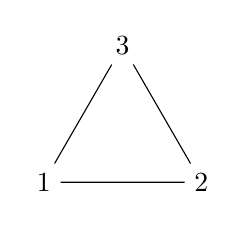
\begin{tikzpicture}[scale=0.5]
      \node (1) at (-2,0) {1};
      \node (2) at (2,0) {2};
      \node (3) at (0,3.4641) {3};
      \draw (1) to (2) to (3) to (1);
    \end{tikzpicture}
  \end{center}


  \begin{enumerate}
  \item List the elements of this group using cycle notation.

    \medskip

    {\bf Answer:}
    \begin{align*}
      \mathrm{id} &= (\phantom{X} )\\
      \mu_1 &= (1,2)\\
      \mu_2 &= (2,3)\\
      \mu_3 &= (1,3)\\
      \rho_1 &= (1,2,3)\\
      \rho_2 &= (1,3,2)
    \end{align*}
    \medskip

  \item What is the order of this group?

    \medskip

    {\bf Answer:} $|G| = 6$.

    \vskip1cm

  \item Is this group cyclic? Is it abelian?\\
    (Give a brief justification for your answers. You may cite 4(b).)

    \medskip
        
    {\bf Answer:} The group $G$ above is {\bf not abelian}.
    Indeed, there is at least one pair of
    noncommuting elements. For example, $\mu_1 \cdot \mu_2 = (1,2)(2,3) = (1,2,3)$, while
    $\mu_2 \cdot \mu_1 = (2,3)(1,2) = (1,3,2)$. Therefore,
    $\mu_1 \cdot \mu_2 \neq \mu_2 \cdot \mu_1$.

    The group $G$ above is {\bf not cyclic}.
    Indeed, recall that every cyclic group is abelian (See Problem 4(b).)
    Therefore, since $G$ is nonabelian, it is not cyclic.
  \end{enumerate}

%%%%%%%%%%%%%%%%%%%%%%%%%%%%%%%%%%%%%%%%%%%%%%%%%%%%%%%%%%%%%%%%%%%%%%%%%%%
  \newpage

\item Suppose $H$ and $K$ are subgroups of a group $G$. Prove or disprove the following:
  \begin{enumerate}
  \item $H\cap K$ is a subgroup of $G$.

    \medskip
    {\bf Claim:} $H\cap K$ is a subgroup of $G$.

    \medskip    

    {\bf Proof:}
    Let $I = H\cap K$. We check that $I$ is a subgroup of $G$.
    Proposition 3.9 states that this is equivalent to showing that $I$ is closed
    under the three operations (nullary, unary, binary) of $G$.  In other words,
    we must show that $I$ contains the identity (the nullary op), 
    $I$ is closed under inverse (the unary op), and
    $I$ is closed under multiplication (the binary op). 
    \begin{itemize}
    \item  (nullary closure) Clearly $e\in I$ since both $H$ and $K$, being themselves
      subgroups, contain $e$.
    \item (unary closure) If $x\in I= H\cap K$, then
      $x \in H$ and $H$ is a subgroup, so $x^{-1}\in H$.
      Similarly, $x \in K$ and $K$ a subgroup implies $x^{-1}\in K$.
      Therefore, $x^{-1} \in H \cap K$.
    \item (binary closure) Suppose $x$ and $y$ belong to $H\cap K$.
      Then, since $x, y \in H$ and $H$ is a subgroup, we have $xy \in H$.
      Similarly, $x, y \in K$ and $K$ a subgroup implies $xy \in K$.  Therefore, 
      $xy \in H\cap K$.
    \end{itemize}

    \bigskip

  \item $H\cup K$ is a subgroup of $G$.

    \medskip
    This is false, and counterexamples abound.
    Here are two:

\medskip

    {\bf Example 1:}
    In the symmetry group of the triangle from Problem 2 above, let 
    $H = \<\mu_1\> = \{\mathrm{id}, \mu_1\}$ and 
    $K = \<\mu_2\> = \{\mathrm{id}, \mu_2\}$.  
    Then the set $H\cup K = \{\mathrm{id}, \mu_1, \mu_2\}$ is not a subgroup
    since it is not closed under the binary operation: 
    $\mu_1 \cdot \mu_2 = \rho_1\notin H\cup K$. 

\medskip

    {\bf Example 2:}
    In the group $\Z_3 \times \Z_3$ that appears in Exercise~33 of Chapter 3, we
    found that $\<(0,1)\> \cup \<(1,0)\> = \{(0,0), (0,1), (0,2), (1,0), (2,0)\},$
    which clearly is not closed under the binary operation of 
    addition modulo 3.  For instance, $(0,1) + (1,0) = (1,1)$ which does not belong
    to the union.
 
\vskip1cm

(See also: Homework 4, Exercises 3.44, 3.45.)
  \end{enumerate}
  \newpage

\item %Let $\mathbf{G} = \<G, \cdot, ^{-1}, e\>$ 
  Let $G$ be a group.  Prove the following:
  \begin{enumerate}
  \item $G$ is abelian if and only if $(gh)^2 = g^2h^2$ holds for all $g, h \in G$.

    \medskip

    {\it Proof:}\\
    ($\Rightarrow$) Suppose $G$ is abelian.  Then for all $g, h \in G$ we have 
    \[
    (gh)^2 = (gh)(gh) = ghgh = gghh = g^2h^2.
    \]
    ($\Leftarrow$) Suppose $(gh)^2 = g^2h^2$ holds for all $g, h \in G$. 
    Fix an arbitrary pair of elements $g, h \in G$.  We must show that
    $gh = hg$. By assumption, $(gh)^2 = g^2h^2$, that is
    \begin{equation}
      \label{eq:1}
    (gh)(gh) =  (gg)(hh).
    \end{equation}
    Multiplying both sides of~(\ref{eq:1}) on the left by $g^{-1}$ and on the
    right by $h^{-1}$, we have
    \begin{equation}
      \label{eq:2}
      g^{-1}(gh)(gh)h^{-1} = g^{-1}(gg)(hh)h^{-1}.
    \end{equation}
    By associativity, the left hand side of~(\ref{eq:2}) is
    $g^{-1}g \, hg \,hh^{-1} = e\, hg\, e = hg$, while the right hand side 
    is
    $g^{-1}g \, gh \,hh^{-1} = e\, gh\, e = gh$.
    Therefore, $hg = gh$. 

    \vskip1cm

  \item If $G$ is cyclic, then $G$ is abelian.

    \medskip

    {\it Proof:}\\
    Suppose $G$ is cyclic.  Then $G = \<a\>$ for some $a \in G$.
    Fix an arbitrary pair of elements $g, h \in G$.  We must show that
    $gh = hg$.  Since $G = \<a\>$, we have $g = a^j$ for some $j\in \N$ and 
    $h = a^k$ for some $k\in \N$.  Therefore, 
    \[
    gh = a^j a^k = a^{j+k} = a^{k+j} = hg.
    \]

    \vskip1cm

  \item Give a specific example of a group $G$ and elements $g, h \in G$ for which $(gh)^2 \neq g^2h^2$. 
    (Justify your answer.)

    \medskip

    {\bf Answer:} Again, the group of symmetries on a triangle that showed up in
    Problem 2 is an example.  Let $g = \mu_1$ and $h = \mu_2$.  Then
    $\mu_1^2 = \mathrm{id} = \mu_2^2$ and $\mu_1 \,\mu_2 = \rho_1$, so,
    \[
    (\mu_1\, \mu_2)^2 = \rho_1^2 = \rho_2 \neq \mathrm{id} = \mu_1^2 \, \mu_2^2.
    \]

    \vskip1cm
  
  \item Give a specific example of a group that is abelian but not cyclic.\\
    (No justification necessary.)

    \medskip

    {\bf Answer:} Many direct products of cyclic groups are abelian but not
    cyclic.  For example, $\Z_2 \times \Z_2$ and $\Z_3 \times \Z_3$ are both
    abelian but not cyclic. 

    (On the other hand, the group $\Z_3 \times \Z_4$ is
    not only abelian, but also cyclic! Check that the element $(1,1)$ generates
    $\Z_3 \times \Z_4$. We will soon see that $\Z_3 \times \Z_4$ is
    just a ``copy'' of the cyclic group $\Z_{12}$, whereas $\Z_2 \times \Z_2$ is truly
    distinct from $\Z_4$.)
  \end{enumerate}

  \newpage
\item This problem has several parts.
  First, state the following (without proof):
  \begin{enumerate}
  \item \emph{The Well Ordering Principle.} (about subsets of natural numbers)

    \medskip

    {\bf Answer:} Every nonempty subset of the natural numbers is well ordered.

\vskip1cm

  \item \emph{The Division Algorithm.} (about integers $a$ and $b$ where $b>0$)

    \medskip

    {\bf Answer:} If $a$ and $b$ are integers and $b>0$, then there exist integers
    $q, r$ such that $a = qb+r$ and $0\leq r < b$. 


    \vskip1cm

    Prove that every subgroup of a cyclic group is cyclic by following the steps below.
    First, let $G = \<a\>$ be a cyclic group and fix an arbitrary subgroup $H\leq G$.

    \medskip

  \item Suppose $H$ contains only the identity, $e$. Say why $H$
    must be cyclic in this case. (one line/sentence)

    \medskip

    {\bf Answer:} $H = \{e\} = \<e\>$ is one-generated, that is, cyclic.

    \vskip1cm

  \item Suppose instead that $H$ contains more than just the identity element. 
    Let $m$ be the smallest positive integer such that $a^m\in H$.  
    Why does such a number $m$ exists? (Hint: consider the set 
    $\{m \in \N: a^m \in H\}$; cite a well known principle; say
    why it applies here.)

    \medskip

    {\bf Answer:} 
    The set $\{m \in \N: a^m \in H\}$ is a subset of the natural numbers.
    We assumed $H$ contains more than just the identity, so there is some 
    $x \in H$ with $x \neq e$.  Since $x \in H \leq G = \<a\>$, there is some
    $m$ such that $x = a^m$. Therefore, the set $\{m \in \N: a^m \in H\}$ is
    nonempty, so it satisfies the hypotheses of the Well Ordering Principle,
    which states that it must be well ordered (i.e., have a least element). 

    \vskip1cm

  \item Finally, prove the {\bf Claim} stated on the {\bf next page}. $\rightarrow$ \\
    (which says that $a^m$ generates $H$, where $m$ is the number from part (b)).
    %% ; that is, prove that if $x$ is an arbitrary element of $H$, then
    %%     $x$ is a power of $a^m$.
  \end{enumerate}

  \newpage
      {\bf Claim:} If $H\leq G = \<a\>$ and $m$ is the smallest positive integer such
      that $a^m \in H$, then $H = \<a^m\>$.

      \medskip

      \noindent {\it Proof:} Let $x \in H$.  The claim is that $a^m$ generates
      $H$, so we need to prove that $x = a^{mq}$ for some $q \in \N$.  
      Since $x \in H \leq G = \<a\>$, we have $x = a^j$ for some $j$, and it
      suffices to show that $m$ divides $j$
      (since this will give $qm = j$ for some $q$, whence
      $x= a^j = a^{qm}$).

      By the division algorithm, there exist integers $q, r$ such that 
      $j = qm + r$ where $0\leq r < m$.  Therefore, 
      \[
      x = a^j = a^{qm+r} = a^{qm}a^r, \quad \text{ so } \quad a^{-qm}x = a^r.
      \]
      Now note that $a^{-qm} \in H$ and $x \in H$ together imply that $a^r \in H$. 
      But $0\leq r < m$ and $m$ is the smallest positive integer with $a^m \in H$. 
      Therefore, $r = 0$, so $j = qm$, and this proves that $m\divides j$.

      \newpage
    \item
      Answer either (a) or (b). Only one answer will be graded.  (If
      you answer both, then clearly mark which should be graded.)
      \begin{enumerate}
      \item 
        Show that, for any cyclic group $G = \<a\>$, 
        the subgroup $\<a^j, a^k\>$ generated by $a^j$ and $a^k$ is equal to
        $\<a^d\>$, where $d = \gcd(j,k)$.
        (Hint: Recall that there exist integers $r$ and $s$ such that $d = rj + sk$; you
        may use this fact without proving it.)
      \item
        Show that for any group $G$, and any fixed element $g \in G$,
        the map $\lambda_g : G \rightarrow G$ defined by
        $\lambda_g(a) = g a$ is a permutation of $G$.
        Then show that the order of the alternating group on $n$ letters is $|A_n| = n!/2$.
        %% (Hint: first explain why the order of $S_n$ is $n!$, then prove that exactly half
        %% of the elements of $S_n$ must be in $A_n$.)
      \end{enumerate}

    \medskip

    \begin{enumerate}
    \item {\bf Claim:} $\<a^d\> = \<a^j, a^k\>$

    \medskip

    {\it Proof:}
    We first show $\<a^d\> \subseteq \<a^j, a^k\>$.
    Since $a^d = a^{rj+sk} = a^{rj}a^{sk} = (a^j)^r(a^k)^s$, we see that 
    $a^d \in \<a^j, a^k\>$, therefore, 
    $\<a^d\> \subseteq \<a^j, a^k\>$.
    
    Next we show $\<a^j, a^k\> \subseteq \<a^d\>$.  
    Since $d = \gcd(j,k)$ we
    have $d \divides j$ so $j = md$ for some integer $m$.  Therefore, 
    $a^j = a^{dm} \in \<a^d\>$.
    Similarly, $d \divides k$ so $k = nd$ for some integer $n$.  Therefore, 
    $a^k = a^{dn} \in \<a^d\>$. Since $a^j$ and $a^k$ both belong to $\<a^d\>$,
    it follows that $\<a^j, a^k\> \subseteq \<a^d\>$.  

    \vskip1cm

  \item
{\bf Claim:}  For any group $G$, and any fixed element $g \in G$,
        the map $\lambda_g : G \rightarrow G$ defined by
        $\lambda_g(a) = g a$ is a permutation of $G$.

        \medskip

        {\it Proof:} We must show that $\lambda_g$ is one-to-one and onto.  Let
        $x, y \in G$ and suppose $\lambda_g(x) = \lambda_g(y)$.  Then $gx = gy$,
        so multiplying on the left of both sides by $g^{-1}$ we have
        $g^{-1}gx = g^{-1}gy$, that is,  $x = y$.  This proves that $\lambda_g$
        is one-to-one.  Let $z \in G$. To show $\lambda_g$ is onto, we must show
        that there is some $x \in G$ with $\lambda_g(x) = z$. Indeed, take 
        $x = g^{-1}z$.  Then $\lambda_g(x) = \lambda_g(g^{-1}z) = gg^{-1}z = z$.

        \vskip1cm

        {\bf Claim:} The order of the alternating group on $n$ letters is $|A_n| = n!/2$.

        \medskip

        {\it Proof:} We know there are $|S_n| = n!$ permutations in the full
        symmetric group on $n$ letters.  We want to show that half of these are
        even permutations.  
        %% (We will take for granted that the identity element
        %% belongs to $A_n$, that is, $\mathrm{id}$ is an even permutation.)  
        Let $B_n$ denote the set of odd permutations.  Fix
        some transposition  $\tau \in S_n$. Any transposition will do, for
        example, we could choose $\tau = (1,2)$. Then define 
        $\lambda_\tau: A_n \rightarrow B_n$ by 
        $\lambda_\tau(\sigma) = \tau \sigma$.  

        We will prove that
        $\lambda_\tau$ is one-to-one and onto, thus proving that $|A_n| =|B_n|$.  
        Since $S_n$ is the disjoint union of the sets $A_n$ and $B_n$, it will
        follow that exactly half of the permutations in $S_n$ are even and half
        are odd, so that $|A_n| = n!/2$.

        Indeed, let $\sigma, \rho$ be two arbitrary even permutation in $A_n$
        and suppose $\lambda_\tau(\sigma) = \lambda_\tau(\rho)$.  Then
        $\tau\sigma = \tau\rho$, so left multiplying both sides by 
        $\tau^{-1}=\tau$ we have $\sigma = \rho$. 
        This proves that $\lambda_\tau$ is one-to-one.

        Suppose $\mu$ is an arbitrary permutation in $B_n$.  We must show there
        is some permutation $\sigma \in A_n$ such that $\lambda_\tau(\sigma) = \mu$.
        Indeed, select $\sigma = \tau\mu$.  Then 
        $\lambda_\tau(\sigma) = \lambda_\tau(\tau\mu) =\tau\tau\mu = \mu$.  (The
        last equality holds since $\tau$ is a transposition, so 
        $\tau^2 = \mathrm{id}$; that is, $\tau = \tau^{-1}$.)

    \end{enumerate}
      \newpage
    \item
      \begin{enumerate}[(a)]
      \item Give a precise definition of \emph{equivalence relation}, then give an example.

    \medskip

    {\bf Answer:} 
        \vskip5cm
      \item Give a precise definition of \emph{partial order relation}, then give an example.

    \medskip

    {\bf Answer:} 
        \vskip5cm
      \item Let $f:X \rightarrow Y$ be a function and define the relation $\sim$
        on the set $X$ as follows:
        \[
        m \sim n \quad \text{ if and only if } \quad f(m) = f(n)
        \]
        What kind of relation is $\sim$?  (Justify your answer by checking the properties.)

    \medskip

    {\bf Answer:} 


        %% \item Give a precise definition of \emph{total order relation}, then give an example.
        %%   \vskip4cm
        %%   \item Of the three types of relations mentioned above, which of these is
        %%     typically associated with a partition of a set into disjoint subsets?
        %%   \vskip4cm
      \end{enumerate}

      \newpage
\end{enumerate}
\begin{center}
  Extra Credit
\end{center}
\begin{enumerate}
\item[EC 1.] ($6$ points)
  Below I have drawn the subgroup lattice diagrams for the groups $\Z_2$, $\Z_2 \times \Z_2$,
  $\Z_7$, $\Z_{12}$, $\Z_{16}$, $\Z_{30}$, and $S_3$, but I've forgotten which diagram
  go with which group.  I was able to label the first diagram
  correctly.  If you think you can help me label the others, go for it. But
  don't guess! 

  \medskip

  {\it $+1$ point for each correct answer, $-1/2$ point for each incorrect answer.} 
  %\begin{multicols}{2}

  \bigskip

  \begin{center}
    % Z_2
    \begin{tikzpicture}[scale=1.25]
      \node (bot) at (0,0) [draw,circle,inner sep=1pt] {};
      \node (top) at (0,2) [draw,circle,inner sep=1pt] {};
      \draw (bot) to (top);
      \node (G) at (0,-1) {$G = \Z_2$};
      \node (line) at (.1,-1.2) {\underline{\phantom{XXXXXXX}}};
    \end{tikzpicture}
    \hskip3cm
    % Z_7
    \begin{tikzpicture}[scale=1.25]
      \node (bot) at (0,0) [draw,circle,inner sep=1pt] {};
      \node (top) at (0,2) [draw,circle,inner sep=1pt] {};
      \draw (bot) to (top);
      \node (line) at (0,-1.2) {\underline{\phantom{XXXXXXX}}};
    \end{tikzpicture}
    % Z_16
    \hskip3cm
    \begin{tikzpicture}[scale=1.25]
      \node (bot) at (0,0) [draw,circle,inner sep=1pt] {};
      \node (1) at (0,1) [draw,circle,inner sep=1pt] {};
      \node (top) at (0,2) [draw,circle,inner sep=1pt] {};
      \draw (bot) to (1) to (top);
      \node (line) at (0,-1.2) {\underline{\phantom{XXXXXXX}}};
    \end{tikzpicture}
  \end{center}
  \vskip1cm
  \begin{center}
    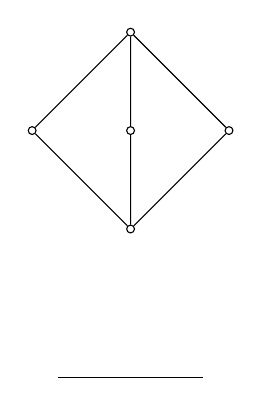
\begin{tikzpicture}[scale=1.25]
      \node (bot) at (0,0) [draw,circle,inner sep=1pt] {};
      \node (1) at (1,1) [draw,circle,inner sep=1pt] {};
      \node (2) at (-1,1) [draw,circle,inner sep=1pt] {};
      \node (3) at (0,1) [draw,circle,inner sep=1pt] {};
      \node (top) at (0,2) [draw,circle,inner sep=1pt] {};
      \draw (bot) to (1) to (top) to (2) to (bot) to (3) to (top);
      \node (line) at (0,-1.4) {\underline{\phantom{XXXXXXX}}};
    \end{tikzpicture}
    \hskip3cm
    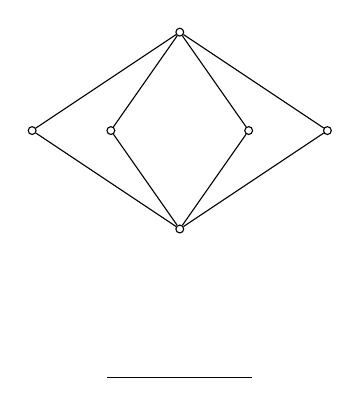
\begin{tikzpicture}[scale=1.25]
      \node (bot) at (0,0) [draw,circle,inner sep=1pt] {};
      \node (1) at (1.5,1) [draw,circle,inner sep=1pt] {};
      \node (2) at (-1.5,1) [draw,circle,inner sep=1pt] {};
      \node (3) at (.7,1) [draw,circle,inner sep=1pt] {};
      \node (4) at (-.7,1) [draw,circle,inner sep=1pt] {};
      \node (top) at (0,2) [draw,circle,inner sep=1pt] {};
      \draw (bot) to (1) to (top) to (2) to (bot) to (3) to (top) to (4) to (bot);
      \node (line) at (0,-1.4) {\underline{\phantom{XXXXXXX}}};
      %  \node (G) at (0,-1.5) {$G =$};
    \end{tikzpicture}
  \end{center}
  \vskip1cm
  \begin{center}
    \begin{tikzpicture}[scale=0.7]
      \node (1) at (0,0) [draw,circle,inner sep=1pt] {};
      \node (6) at (2,2)[draw,circle,inner sep=1pt] {}; 
      \node (4) at (-2,2) [draw,circle,inner sep=1pt] {};
      \node (2) at (0,4) [draw,circle,inner sep=1pt] {};
      \node (3) at (4,4) [draw,circle,inner sep=1pt] {};
      \node (G) at (2,6) [draw,circle,inner sep=1pt] {};
      \draw (1) to (6) to (2) to (4) to (1);
      \draw (6) to (3) to (G) to (2) to (4);
      \node (line) at (1,-1.4) {\underline{\phantom{XXXXXXX}}};
      %  \node (G) at (0,-1.5) {$G =$};
    \end{tikzpicture}
    \hskip3cm
    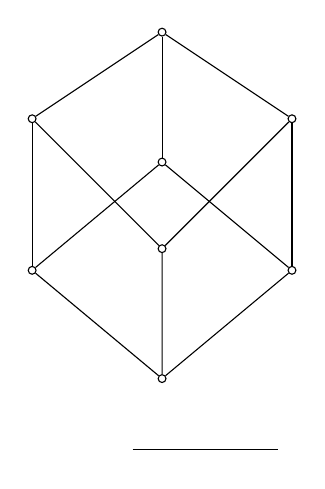
\begin{tikzpicture}[scale=0.55]
      \node (e) at (0,0)  [draw,circle,inner sep=1pt] {};
      \node (G) at (0,8) [draw,circle,inner sep=1pt] {};
      \node (2) at (-3,6) [draw,circle,inner sep=1pt] {};
      \node (3) at (0,5)  [draw,circle,inner sep=1pt] {};
      \node (5) at (3,6) [draw,circle,inner sep=1pt] {}; 
      \node (6) at (-3,2.5) [draw,circle,inner sep=1pt] {};
      \node (10) at (0,3)  [draw,circle,inner sep=1pt] {};
      \node (15) at (3,2.5)  [draw,circle,inner sep=1pt] {};
      \node (line) at (1,-1.4) {\underline{\phantom{XXXXXXX}}};
      \draw (e) to (15) to (3) to (6) to (e);
      \draw (e) to (10) to (5) to (G) to (2) to (10);
      \draw (6) to (2) (3) to (G) (15) to (5);
    \end{tikzpicture}
  \end{center}

\item[EC 2.] (1/2 point) Which group appears in William DeMeo's GitHub gravatar?\\
  {\small (William DeMeo the mathematician, not the actor.)}
\end{enumerate}

\end{document}

